\documentclass[twoside]{book}

% Packages required by doxygen
\usepackage{fixltx2e}
\usepackage{calc}
\usepackage{doxygen}
\usepackage[export]{adjustbox} % also loads graphicx
\usepackage{graphicx}
\usepackage[utf8]{inputenc}
\usepackage{makeidx}
\usepackage{multicol}
\usepackage{multirow}
\PassOptionsToPackage{warn}{textcomp}
\usepackage{textcomp}
\usepackage[nointegrals]{wasysym}
\usepackage[table]{xcolor}

% Font selection
\usepackage[T1]{fontenc}
\usepackage[scaled=.90]{helvet}
\usepackage{courier}
\usepackage{amssymb}
\usepackage{sectsty}
\renewcommand{\familydefault}{\sfdefault}
\allsectionsfont{%
  \fontseries{bc}\selectfont%
  \color{darkgray}%
}
\renewcommand{\DoxyLabelFont}{%
  \fontseries{bc}\selectfont%
  \color{darkgray}%
}
\newcommand{\+}{\discretionary{\mbox{\scriptsize$\hookleftarrow$}}{}{}}

% Page & text layout
\usepackage{geometry}
\geometry{%
  a4paper,%
  top=2.5cm,%
  bottom=2.5cm,%
  left=2.5cm,%
  right=2.5cm%
}
\tolerance=750
\hfuzz=15pt
\hbadness=750
\setlength{\emergencystretch}{15pt}
\setlength{\parindent}{0cm}
\setlength{\parskip}{0.2cm}
\makeatletter
\renewcommand{\paragraph}{%
  \@startsection{paragraph}{4}{0ex}{-1.0ex}{1.0ex}{%
    \normalfont\normalsize\bfseries\SS@parafont%
  }%
}
\renewcommand{\subparagraph}{%
  \@startsection{subparagraph}{5}{0ex}{-1.0ex}{1.0ex}{%
    \normalfont\normalsize\bfseries\SS@subparafont%
  }%
}
\makeatother

% Headers & footers
\usepackage{fancyhdr}
\pagestyle{fancyplain}
\fancyhead[LE]{\fancyplain{}{\bfseries\thepage}}
\fancyhead[CE]{\fancyplain{}{}}
\fancyhead[RE]{\fancyplain{}{\bfseries\leftmark}}
\fancyhead[LO]{\fancyplain{}{\bfseries\rightmark}}
\fancyhead[CO]{\fancyplain{}{}}
\fancyhead[RO]{\fancyplain{}{\bfseries\thepage}}
\fancyfoot[LE]{\fancyplain{}{}}
\fancyfoot[CE]{\fancyplain{}{}}
\fancyfoot[RE]{\fancyplain{}{\bfseries\scriptsize Generated on Sat Apr 25 2015 17\+:55\+:39 for My Project by Doxygen }}
\fancyfoot[LO]{\fancyplain{}{\bfseries\scriptsize Generated on Sat Apr 25 2015 17\+:55\+:39 for My Project by Doxygen }}
\fancyfoot[CO]{\fancyplain{}{}}
\fancyfoot[RO]{\fancyplain{}{}}
\renewcommand{\footrulewidth}{0.4pt}
\renewcommand{\chaptermark}[1]{%
  \markboth{#1}{}%
}
\renewcommand{\sectionmark}[1]{%
  \markright{\thesection\ #1}%
}

% Indices & bibliography
\usepackage{natbib}
\usepackage[titles]{tocloft}
\setcounter{tocdepth}{3}
\setcounter{secnumdepth}{5}
\makeindex

% Hyperlinks (required, but should be loaded last)
\usepackage{ifpdf}
\ifpdf
  \usepackage[pdftex,pagebackref=true]{hyperref}
\else
  \usepackage[ps2pdf,pagebackref=true]{hyperref}
\fi
\hypersetup{%
  colorlinks=true,%
  linkcolor=blue,%
  citecolor=blue,%
  unicode%
}

% Custom commands
\newcommand{\clearemptydoublepage}{%
  \newpage{\pagestyle{empty}\cleardoublepage}%
}


%===== C O N T E N T S =====

\begin{document}

% Titlepage & ToC
\hypersetup{pageanchor=false,
             bookmarks=true,
             bookmarksnumbered=true,
             pdfencoding=unicode
            }
\pagenumbering{roman}
\begin{titlepage}
\vspace*{7cm}
\begin{center}%
{\Large My Project }\\
\vspace*{1cm}
{\large Generated by Doxygen 1.8.9.1}\\
\vspace*{0.5cm}
{\small Sat Apr 25 2015 17:55:39}\\
\end{center}
\end{titlepage}
\clearemptydoublepage
\tableofcontents
\clearemptydoublepage
\pagenumbering{arabic}
\hypersetup{pageanchor=true}

%--- Begin generated contents ---
\chapter{Hierarchical Index}
\section{Class Hierarchy}
This inheritance list is sorted roughly, but not completely, alphabetically\+:\begin{DoxyCompactList}
\item \contentsline{section}{B\+F\+\_\+element\+D\+A\+T\+A}{\pageref{struct_b_f__element_d_a_t_a}}{}
\item \contentsline{section}{B\+F\+\_\+pair$<$ T $>$}{\pageref{struct_b_f__pair}}{}
\item \contentsline{section}{Bn\+B\+\_\+element\+D\+A\+T\+A}{\pageref{struct_bn_b__element_d_a_t_a}}{}
\item \contentsline{section}{Bn\+B\+\_\+node}{\pageref{class_bn_b__node}}{}
\begin{DoxyCompactList}
\item \contentsline{section}{Bn\+B\+\_\+node\+\_\+checked}{\pageref{class_bn_b__node__checked}}{}
\item \contentsline{section}{Bn\+B\+\_\+node\+\_\+not\+Checked}{\pageref{class_bn_b__node__not_checked}}{}
\end{DoxyCompactList}
\item \contentsline{section}{Bn\+B\+\_\+pair$<$ T $>$}{\pageref{struct_bn_b__pair}}{}
\item \contentsline{section}{Bn\+B\+\_\+\+U\+P$<$ T $>$}{\pageref{class_bn_b___u_p}}{}
\item \contentsline{section}{Brute\+Force$<$ T, R $>$}{\pageref{class_brute_force}}{}
\item \contentsline{section}{Brute\+Force\+\_\+node}{\pageref{class_brute_force__node}}{}
\item \contentsline{section}{City}{\pageref{class_city}}{}
\begin{DoxyCompactList}
\item \contentsline{section}{Manchester}{\pageref{class_manchester}}{}
\end{DoxyCompactList}
\item \contentsline{section}{compare\+\_\+\+Bn\+Bnode\+Pointers}{\pageref{structcompare___bn_bnode_pointers}}{}
\item \contentsline{section}{Compare\+Nodes}{\pageref{struct_compare_nodes}}{}
\end{DoxyCompactList}

\chapter{Class Index}
\section{Class List}
Here are the classes, structs, unions and interfaces with brief descriptions\+:\begin{DoxyCompactList}
\item\contentsline{section}{\hyperlink{struct_b_f__element_d_a_t_a}{B\+F\+\_\+element\+D\+A\+T\+A} \\*Stores each element information }{\pageref{struct_b_f__element_d_a_t_a}}{}
\item\contentsline{section}{\hyperlink{struct_b_f__pair}{B\+F\+\_\+pair$<$ T $>$} \\*Creates alias for a type that saves the element data and a pointer to the element inside the B\+F class (not really a needed struct, only used to \char`\"{}simplify\char`\"{} notation) }{\pageref{struct_b_f__pair}}{}
\item\contentsline{section}{\hyperlink{struct_bn_b__element_d_a_t_a}{Bn\+B\+\_\+element\+D\+A\+T\+A} \\*Saves an element\textquotesingle{}s data needed to compute the Bn\+B solution }{\pageref{struct_bn_b__element_d_a_t_a}}{}
\item\contentsline{section}{\hyperlink{class_bn_b__node}{Bn\+B\+\_\+node} \\*Stores Branch and Bound node information }{\pageref{class_bn_b__node}}{}
\item\contentsline{section}{\hyperlink{class_bn_b__node__checked}{Bn\+B\+\_\+node\+\_\+checked} \\*Subclass that indicates that the index of the node as been unchecked }{\pageref{class_bn_b__node__checked}}{}
\item\contentsline{section}{\hyperlink{class_bn_b__node__not_checked}{Bn\+B\+\_\+node\+\_\+not\+Checked} \\*Subclass that indicates that the index of the node as been checked Saves values related to previous calculated bound to speed up the calculation of a new bound }{\pageref{class_bn_b__node__not_checked}}{}
\item\contentsline{section}{\hyperlink{struct_bn_b__pair}{Bn\+B\+\_\+pair$<$ T $>$} \\*Creates alias for a type that saves the element data and a pointer to the element inside the Bn\+B class (not really a needed struct, only used to \char`\"{}simplify\char`\"{} notation) }{\pageref{struct_bn_b__pair}}{}
\item\contentsline{section}{\hyperlink{class_bn_b___u_p}{Bn\+B\+\_\+\+U\+P$<$ T $>$} \\*Branch n Bound implementation, done with max bounds (usually it\textquotesingle{}s done in reverse) }{\pageref{class_bn_b___u_p}}{}
\item\contentsline{section}{\hyperlink{class_brute_force}{Brute\+Force$<$ T, R $>$} \\*Branch n Bound implementation, done with max bounds (usually it\textquotesingle{}s done in reverse) }{\pageref{class_brute_force}}{}
\item\contentsline{section}{\hyperlink{class_brute_force__node}{Brute\+Force\+\_\+node} \\*Stores \hyperlink{class_brute_force}{Brute\+Force} node information }{\pageref{class_brute_force__node}}{}
\item\contentsline{section}{\hyperlink{class_city}{City} }{\pageref{class_city}}{}
\item\contentsline{section}{\hyperlink{structcompare___bn_bnode_pointers}{compare\+\_\+\+Bn\+Bnode\+Pointers} \\*Defines comparison for node pointers, to be used in queue ordering }{\pageref{structcompare___bn_bnode_pointers}}{}
\item\contentsline{section}{\hyperlink{struct_compare_nodes}{Compare\+Nodes} \\*Struct with comparison for nodes. Used in greedy\+Solve(). could help speedup search. not sure though.. }{\pageref{struct_compare_nodes}}{}
\item\contentsline{section}{\hyperlink{class_manchester}{Manchester} }{\pageref{class_manchester}}{}
\end{DoxyCompactList}

\chapter{Class Documentation}
\hypertarget{struct_b_f__element_d_a_t_a}{}\section{B\+F\+\_\+element\+D\+A\+T\+A Struct Reference}
\label{struct_b_f__element_d_a_t_a}\index{B\+F\+\_\+element\+D\+A\+T\+A@{B\+F\+\_\+element\+D\+A\+T\+A}}


stores each element information  




{\ttfamily \#include $<$brute\+Force.\+h$>$}

\subsection*{Public Attributes}
\begin{DoxyCompactItemize}
\item 
\hypertarget{struct_b_f__element_d_a_t_a_ae232c7505bda3893516bf5c06d30757b}{}double {\bfseries cost}\label{struct_b_f__element_d_a_t_a_ae232c7505bda3893516bf5c06d30757b}

\item 
\hypertarget{struct_b_f__element_d_a_t_a_af4765c7ca62b5e581c2523f38c18257e}{}double {\bfseries value}\label{struct_b_f__element_d_a_t_a_af4765c7ca62b5e581c2523f38c18257e}

\end{DoxyCompactItemize}


\subsection{Detailed Description}
stores each element information 

The documentation for this struct was generated from the following file\+:\begin{DoxyCompactItemize}
\item 
brute\+Force.\+h\end{DoxyCompactItemize}

\hypertarget{struct_b_f__pair}{}\section{B\+F\+\_\+pair$<$ T $>$ Struct Template Reference}
\label{struct_b_f__pair}\index{B\+F\+\_\+pair$<$ T $>$@{B\+F\+\_\+pair$<$ T $>$}}


creates alias for a type that saves the element data and a pointer to the element inside the B\+F class (not really a needed struct, only used to \char`\"{}simplify\char`\"{} notation)  




{\ttfamily \#include $<$brute\+Force.\+h$>$}

\subsection*{Public Types}
\begin{DoxyCompactItemize}
\item 
\hypertarget{struct_b_f__pair_ae2be33ae51bdd93073f24e48b63deff1}{}typedef pair$<$ \hyperlink{struct_b_f__element_d_a_t_a}{B\+F\+\_\+element\+D\+A\+T\+A}, T $\ast$ $>$ {\bfseries type\+T}\label{struct_b_f__pair_ae2be33ae51bdd93073f24e48b63deff1}

\end{DoxyCompactItemize}


\subsection{Detailed Description}
\subsubsection*{template$<$typename T$>$struct B\+F\+\_\+pair$<$ T $>$}

creates alias for a type that saves the element data and a pointer to the element inside the B\+F class (not really a needed struct, only used to \char`\"{}simplify\char`\"{} notation) 

The documentation for this struct was generated from the following file\+:\begin{DoxyCompactItemize}
\item 
brute\+Force.\+h\end{DoxyCompactItemize}

\hypertarget{struct_bn_b__element_d_a_t_a}{}\section{Bn\+B\+\_\+element\+D\+A\+T\+A Struct Reference}
\label{struct_bn_b__element_d_a_t_a}\index{Bn\+B\+\_\+element\+D\+A\+T\+A@{Bn\+B\+\_\+element\+D\+A\+T\+A}}


Saves an element\textquotesingle{}s data needed to compute the Bn\+B solution.  




{\ttfamily \#include $<$generic\+Bn\+B.\+h$>$}

\subsection*{Public Attributes}
\begin{DoxyCompactItemize}
\item 
\hypertarget{struct_bn_b__element_d_a_t_a_ad2924da6deff21e31ced39f3e5aae097}{}double \hyperlink{struct_bn_b__element_d_a_t_a_ad2924da6deff21e31ced39f3e5aae097}{cost}\label{struct_bn_b__element_d_a_t_a_ad2924da6deff21e31ced39f3e5aae097}

\begin{DoxyCompactList}\small\item\em element evaluated cost \end{DoxyCompactList}\item 
\hypertarget{struct_bn_b__element_d_a_t_a_a87d3d0845c9aaa362ce98e34f329dde9}{}double \hyperlink{struct_bn_b__element_d_a_t_a_a87d3d0845c9aaa362ce98e34f329dde9}{value}\label{struct_bn_b__element_d_a_t_a_a87d3d0845c9aaa362ce98e34f329dde9}

\begin{DoxyCompactList}\small\item\em element evaluated value \end{DoxyCompactList}\item 
\hypertarget{struct_bn_b__element_d_a_t_a_af80eb28f770d18ac07957be349c2c971}{}double \hyperlink{struct_bn_b__element_d_a_t_a_af80eb28f770d18ac07957be349c2c971}{value\+\_\+cost\+\_\+ratio}\label{struct_bn_b__element_d_a_t_a_af80eb28f770d18ac07957be349c2c971}

\begin{DoxyCompactList}\small\item\em ratio = element value / element cost \end{DoxyCompactList}\end{DoxyCompactItemize}


\subsection{Detailed Description}
Saves an element\textquotesingle{}s data needed to compute the Bn\+B solution. 

The documentation for this struct was generated from the following file\+:\begin{DoxyCompactItemize}
\item 
generic\+Bn\+B.\+h\end{DoxyCompactItemize}

\hypertarget{class_bn_b__node}{}\section{Bn\+B\+\_\+node Class Reference}
\label{class_bn_b__node}\index{Bn\+B\+\_\+node@{Bn\+B\+\_\+node}}


Stores Branch and Bound node information.  




{\ttfamily \#include $<$generic\+Bn\+B.\+h$>$}

Inheritance diagram for Bn\+B\+\_\+node\+:\begin{figure}[H]
\begin{center}
\leavevmode
\includegraphics[height=2.000000cm]{class_bn_b__node}
\end{center}
\end{figure}
\subsection*{Public Member Functions}
\begin{DoxyCompactItemize}
\item 
\hypertarget{class_bn_b__node_a59c19a1a90773b24e175fc7ff2a5d7a5}{}{\bfseries Bn\+B\+\_\+node} (double \hyperlink{class_bn_b__node_a6a44afc83f3d0c1601804b61cf03fbf1}{cost}, double \hyperlink{class_bn_b__node_a726b74bbceb33532ee8678e0722d62aa}{value}, double \hyperlink{class_bn_b__node_a275b8c6f02b922e74a7f82d8fb3b5cf9}{bound}, int \hyperlink{class_bn_b__node_a531520424d5cc944a542a984cc14f32f}{index}, \hyperlink{class_bn_b__node}{Bn\+B\+\_\+node} $\ast$\hyperlink{class_bn_b__node_ac70c63a5ed68adefb9bc9540ac8e68dd}{parent})\label{class_bn_b__node_a59c19a1a90773b24e175fc7ff2a5d7a5}

\item 
virtual bool \hyperlink{class_bn_b__node_ae59aee037f8c7c88b9b63948e7b5d8cb}{checked} ()=0
\begin{DoxyCompactList}\small\item\em Checks if a node is checked or unchecked. \end{DoxyCompactList}\end{DoxyCompactItemize}
\subsection*{Public Attributes}
\begin{DoxyCompactItemize}
\item 
\hypertarget{class_bn_b__node_a6a44afc83f3d0c1601804b61cf03fbf1}{}double \hyperlink{class_bn_b__node_a6a44afc83f3d0c1601804b61cf03fbf1}{cost}\label{class_bn_b__node_a6a44afc83f3d0c1601804b61cf03fbf1}

\begin{DoxyCompactList}\small\item\em sum of all the checked items (indexes in parent\+Nodes) cost plus cost of element at index $<$index$>$ if the node is checked \end{DoxyCompactList}\item 
\hypertarget{class_bn_b__node_a726b74bbceb33532ee8678e0722d62aa}{}double \hyperlink{class_bn_b__node_a726b74bbceb33532ee8678e0722d62aa}{value}\label{class_bn_b__node_a726b74bbceb33532ee8678e0722d62aa}

\begin{DoxyCompactList}\small\item\em same as cost but done with the values of the elements \end{DoxyCompactList}\item 
\hypertarget{class_bn_b__node_a275b8c6f02b922e74a7f82d8fb3b5cf9}{}double \hyperlink{class_bn_b__node_a275b8c6f02b922e74a7f82d8fb3b5cf9}{bound}\label{class_bn_b__node_a275b8c6f02b922e74a7f82d8fb3b5cf9}

\begin{DoxyCompactList}\small\item\em the max/min bound calculated for the current node (the current implementation uses max bounds) \end{DoxyCompactList}\item 
\hypertarget{class_bn_b__node_a531520424d5cc944a542a984cc14f32f}{}int \hyperlink{class_bn_b__node_a531520424d5cc944a542a984cc14f32f}{index}\label{class_bn_b__node_a531520424d5cc944a542a984cc14f32f}

\begin{DoxyCompactList}\small\item\em index of the un/checked item. \end{DoxyCompactList}\item 
\hypertarget{class_bn_b__node_ac70c63a5ed68adefb9bc9540ac8e68dd}{}\hyperlink{class_bn_b__node}{Bn\+B\+\_\+node} $\ast$ \hyperlink{class_bn_b__node_ac70c63a5ed68adefb9bc9540ac8e68dd}{parent}\label{class_bn_b__node_ac70c63a5ed68adefb9bc9540ac8e68dd}

\begin{DoxyCompactList}\small\item\em the parent node. should be N\+U\+L\+L if is first node. \end{DoxyCompactList}\end{DoxyCompactItemize}


\subsection{Detailed Description}
Stores Branch and Bound node information. 

\subsection{Member Function Documentation}
\hypertarget{class_bn_b__node_ae59aee037f8c7c88b9b63948e7b5d8cb}{}\index{Bn\+B\+\_\+node@{Bn\+B\+\_\+node}!checked@{checked}}
\index{checked@{checked}!Bn\+B\+\_\+node@{Bn\+B\+\_\+node}}
\subsubsection[{checked}]{\setlength{\rightskip}{0pt plus 5cm}virtual bool Bn\+B\+\_\+node\+::checked (
\begin{DoxyParamCaption}
{}
\end{DoxyParamCaption}
)\hspace{0.3cm}{\ttfamily [pure virtual]}}\label{class_bn_b__node_ae59aee037f8c7c88b9b63948e7b5d8cb}


Checks if a node is checked or unchecked. 

\begin{DoxyReturn}{Returns}
true if checked, false otherwise 
\end{DoxyReturn}


Implemented in \hyperlink{class_bn_b__node__not_checked_a470c31c7d9f0cce678a2d9074a481407}{Bn\+B\+\_\+node\+\_\+not\+Checked}, and \hyperlink{class_bn_b__node__checked_ab4f7550e430ffa2451386045a4dce9f8}{Bn\+B\+\_\+node\+\_\+checked}.



The documentation for this class was generated from the following file\+:\begin{DoxyCompactItemize}
\item 
generic\+Bn\+B.\+h\end{DoxyCompactItemize}

\hypertarget{class_bn_b__node__checked}{}\section{Bn\+B\+\_\+node\+\_\+checked Class Reference}
\label{class_bn_b__node__checked}\index{Bn\+B\+\_\+node\+\_\+checked@{Bn\+B\+\_\+node\+\_\+checked}}


Subclass that indicates that the index of the node as been unchecked.  




{\ttfamily \#include $<$generic\+Bn\+B.\+h$>$}

Inheritance diagram for Bn\+B\+\_\+node\+\_\+checked\+:\begin{figure}[H]
\begin{center}
\leavevmode
\includegraphics[height=2.000000cm]{class_bn_b__node__checked}
\end{center}
\end{figure}
\subsection*{Public Member Functions}
\begin{DoxyCompactItemize}
\item 
bool \hyperlink{class_bn_b__node__checked_ab4f7550e430ffa2451386045a4dce9f8}{checked} ()
\begin{DoxyCompactList}\small\item\em Checks if a node is checked or unchecked. \end{DoxyCompactList}\item 
\hypertarget{class_bn_b__node__checked_ae0c755ab3273803bc467d9feb0670646}{}{\bfseries Bn\+B\+\_\+node\+\_\+checked} (double \hyperlink{class_bn_b__node_a6a44afc83f3d0c1601804b61cf03fbf1}{cost}, double \hyperlink{class_bn_b__node_a726b74bbceb33532ee8678e0722d62aa}{value}, double \hyperlink{class_bn_b__node_a275b8c6f02b922e74a7f82d8fb3b5cf9}{bound}, int \hyperlink{class_bn_b__node_a531520424d5cc944a542a984cc14f32f}{index}, \hyperlink{class_bn_b__node}{Bn\+B\+\_\+node} $\ast$\hyperlink{class_bn_b__node_ac70c63a5ed68adefb9bc9540ac8e68dd}{parent})\label{class_bn_b__node__checked_ae0c755ab3273803bc467d9feb0670646}

\end{DoxyCompactItemize}
\subsection*{Additional Inherited Members}


\subsection{Detailed Description}
Subclass that indicates that the index of the node as been unchecked. 

\subsection{Member Function Documentation}
\hypertarget{class_bn_b__node__checked_ab4f7550e430ffa2451386045a4dce9f8}{}\index{Bn\+B\+\_\+node\+\_\+checked@{Bn\+B\+\_\+node\+\_\+checked}!checked@{checked}}
\index{checked@{checked}!Bn\+B\+\_\+node\+\_\+checked@{Bn\+B\+\_\+node\+\_\+checked}}
\subsubsection[{checked}]{\setlength{\rightskip}{0pt plus 5cm}bool Bn\+B\+\_\+node\+\_\+checked\+::checked (
\begin{DoxyParamCaption}
{}
\end{DoxyParamCaption}
)\hspace{0.3cm}{\ttfamily [inline]}, {\ttfamily [virtual]}}\label{class_bn_b__node__checked_ab4f7550e430ffa2451386045a4dce9f8}


Checks if a node is checked or unchecked. 

\begin{DoxyReturn}{Returns}
true if checked, false otherwise 
\end{DoxyReturn}


Implements \hyperlink{class_bn_b__node_ae59aee037f8c7c88b9b63948e7b5d8cb}{Bn\+B\+\_\+node}.



The documentation for this class was generated from the following file\+:\begin{DoxyCompactItemize}
\item 
generic\+Bn\+B.\+h\end{DoxyCompactItemize}

\hypertarget{class_bn_b__node__not_checked}{}\section{Bn\+B\+\_\+node\+\_\+not\+Checked Class Reference}
\label{class_bn_b__node__not_checked}\index{Bn\+B\+\_\+node\+\_\+not\+Checked@{Bn\+B\+\_\+node\+\_\+not\+Checked}}


Subclass that indicates that the index of the node as been checked Saves values related to previous calculated bound to speed up the calculation of a new bound.  




{\ttfamily \#include $<$generic\+Bn\+B.\+h$>$}

Inheritance diagram for Bn\+B\+\_\+node\+\_\+not\+Checked\+:\begin{figure}[H]
\begin{center}
\leavevmode
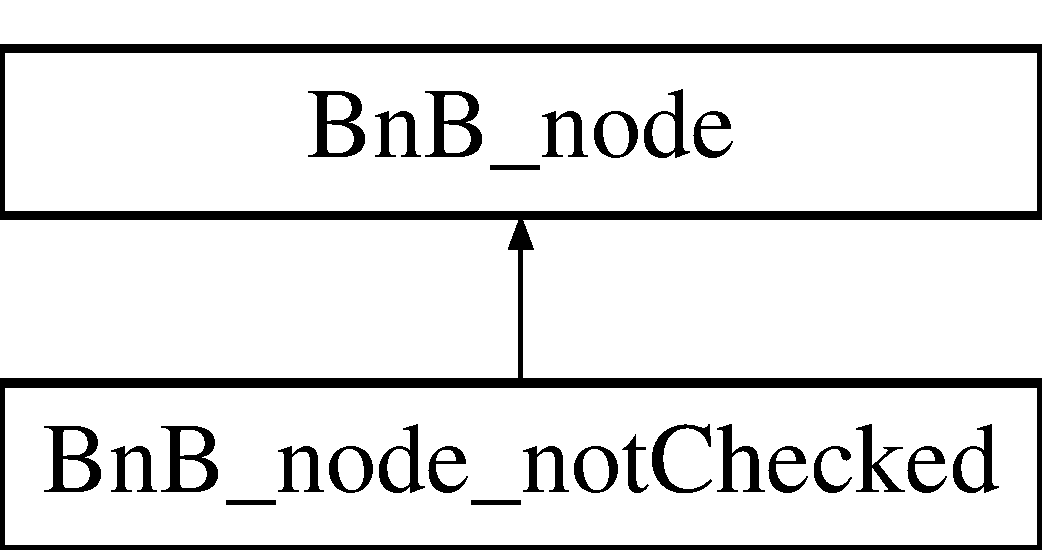
\includegraphics[height=2.000000cm]{class_bn_b__node__not_checked}
\end{center}
\end{figure}
\subsection*{Public Member Functions}
\begin{DoxyCompactItemize}
\item 
bool \hyperlink{class_bn_b__node__not_checked_a470c31c7d9f0cce678a2d9074a481407}{checked} ()
\begin{DoxyCompactList}\small\item\em Checks if a node is checked or unchecked. \end{DoxyCompactList}\item 
\hypertarget{class_bn_b__node__not_checked_a9bd7b93617b59a61e24e663478552b98}{}{\bfseries Bn\+B\+\_\+node\+\_\+not\+Checked} (double \hyperlink{class_bn_b__node_a6a44afc83f3d0c1601804b61cf03fbf1}{cost}, double \hyperlink{class_bn_b__node_a726b74bbceb33532ee8678e0722d62aa}{value}, double \hyperlink{class_bn_b__node_a275b8c6f02b922e74a7f82d8fb3b5cf9}{bound}, int \hyperlink{class_bn_b__node_a531520424d5cc944a542a984cc14f32f}{index}, \hyperlink{class_bn_b__node}{Bn\+B\+\_\+node} $\ast$\hyperlink{class_bn_b__node_ac70c63a5ed68adefb9bc9540ac8e68dd}{parent}, int liib\+Index, double liib\+Cost\+Used)\label{class_bn_b__node__not_checked_a9bd7b93617b59a61e24e663478552b98}

\end{DoxyCompactItemize}
\subsection*{Public Attributes}
\begin{DoxyCompactItemize}
\item 
\hypertarget{class_bn_b__node__not_checked_ad552ee24485d0f9f2f2d2481a6fdbfe4}{}int \hyperlink{class_bn_b__node__not_checked_ad552ee24485d0f9f2f2d2481a6fdbfe4}{last\+Item\+In\+Bound\+Index}\label{class_bn_b__node__not_checked_ad552ee24485d0f9f2f2d2481a6fdbfe4}

\begin{DoxyCompactList}\small\item\em index of the last item used to calculate the previous bound \end{DoxyCompactList}\item 
\hypertarget{class_bn_b__node__not_checked_aa3dc272166a29543020ffc37fe82f9d4}{}double \hyperlink{class_bn_b__node__not_checked_aa3dc272166a29543020ffc37fe82f9d4}{last\+Item\+In\+Bound\+Cost\+Used}\label{class_bn_b__node__not_checked_aa3dc272166a29543020ffc37fe82f9d4}

\begin{DoxyCompactList}\small\item\em the part of the cost used by the element at index $<$index$>$ in previous bound calculation (might be less than the actual element cost) \end{DoxyCompactList}\end{DoxyCompactItemize}


\subsection{Detailed Description}
Subclass that indicates that the index of the node as been checked Saves values related to previous calculated bound to speed up the calculation of a new bound. 

\subsection{Member Function Documentation}
\hypertarget{class_bn_b__node__not_checked_a470c31c7d9f0cce678a2d9074a481407}{}\index{Bn\+B\+\_\+node\+\_\+not\+Checked@{Bn\+B\+\_\+node\+\_\+not\+Checked}!checked@{checked}}
\index{checked@{checked}!Bn\+B\+\_\+node\+\_\+not\+Checked@{Bn\+B\+\_\+node\+\_\+not\+Checked}}
\subsubsection[{checked}]{\setlength{\rightskip}{0pt plus 5cm}bool Bn\+B\+\_\+node\+\_\+not\+Checked\+::checked (
\begin{DoxyParamCaption}
{}
\end{DoxyParamCaption}
)\hspace{0.3cm}{\ttfamily [inline]}, {\ttfamily [virtual]}}\label{class_bn_b__node__not_checked_a470c31c7d9f0cce678a2d9074a481407}


Checks if a node is checked or unchecked. 

\begin{DoxyReturn}{Returns}
true if checked, false otherwise 
\end{DoxyReturn}


Implements \hyperlink{class_bn_b__node_ae59aee037f8c7c88b9b63948e7b5d8cb}{Bn\+B\+\_\+node}.



The documentation for this class was generated from the following file\+:\begin{DoxyCompactItemize}
\item 
generic\+Bn\+B.\+h\end{DoxyCompactItemize}

\hypertarget{struct_bn_b__pair}{}\section{Bn\+B\+\_\+pair$<$ T $>$ Struct Template Reference}
\label{struct_bn_b__pair}\index{Bn\+B\+\_\+pair$<$ T $>$@{Bn\+B\+\_\+pair$<$ T $>$}}


creates alias for a type that saves the element data and a pointer to the element inside the Bn\+B class (not really a needed struct, only used to \char`\"{}simplify\char`\"{} notation)  




{\ttfamily \#include $<$generic\+Bn\+B.\+h$>$}

\subsection*{Public Types}
\begin{DoxyCompactItemize}
\item 
\hypertarget{struct_bn_b__pair_a1fc06192d7cc8297619806b35f452a6d}{}typedef pair$<$ \hyperlink{struct_bn_b__element_d_a_t_a}{Bn\+B\+\_\+element\+D\+A\+T\+A}, T $\ast$ $>$ {\bfseries type\+T}\label{struct_bn_b__pair_a1fc06192d7cc8297619806b35f452a6d}

\end{DoxyCompactItemize}


\subsection{Detailed Description}
\subsubsection*{template$<$typename T$>$struct Bn\+B\+\_\+pair$<$ T $>$}

creates alias for a type that saves the element data and a pointer to the element inside the Bn\+B class (not really a needed struct, only used to \char`\"{}simplify\char`\"{} notation) 

The documentation for this struct was generated from the following file\+:\begin{DoxyCompactItemize}
\item 
generic\+Bn\+B.\+h\end{DoxyCompactItemize}

\hypertarget{class_bn_b___u_p}{}\section{Bn\+B\+\_\+\+U\+P$<$ T $>$ Class Template Reference}
\label{class_bn_b___u_p}\index{Bn\+B\+\_\+\+U\+P$<$ T $>$@{Bn\+B\+\_\+\+U\+P$<$ T $>$}}


Branch n Bound implementation, done with max bounds (usually it\textquotesingle{}s done in reverse)  




{\ttfamily \#include $<$generic\+Bn\+B.\+h$>$}

\subsection*{Public Member Functions}
\begin{DoxyCompactItemize}
\item 
\hypertarget{class_bn_b___u_p_a1906f95c4d3eb96568d6f314e2878808}{}{\bfseries Bn\+B\+\_\+\+U\+P} (vector$<$ T $>$ \&elements, double \hyperlink{class_bn_b___u_p_a0749a907c11c880f825fd0644a8a2bfd}{max\+Cost}, double(T\+::$\ast$get\+Cost)(void), double(T\+::$\ast$get\+Value)(void))\label{class_bn_b___u_p_a1906f95c4d3eb96568d6f314e2878808}

\item 
\hypertarget{class_bn_b___u_p_ae26455243268d49878421014d4bc1645}{}{\bfseries Bn\+B\+\_\+\+U\+P} (vector$<$ T $\ast$ $>$ \&elements, double \hyperlink{class_bn_b___u_p_a0749a907c11c880f825fd0644a8a2bfd}{max\+Cost}, void(T\+::$\ast$get\+Cost)(void), void(T\+::$\ast$get\+Value)(void))\label{class_bn_b___u_p_ae26455243268d49878421014d4bc1645}

\item 
double \hyperlink{class_bn_b___u_p_a52efbfa978fd9b6c43e50da878862d93}{find\+Upper\+Bound\+\_\+1} (\hyperlink{class_bn_b__node}{Bn\+B\+\_\+node} $\ast$node, int $\ast$last\+Item\+In\+Bound\+Index, double $\ast$lat\+Item\+In\+Bound\+Cost\+Used)
\begin{DoxyCompactList}\small\item\em Find new upper bound. Called only when uncheking. \end{DoxyCompactList}\item 
vector$<$ T $\ast$ $>$ \hyperlink{class_bn_b___u_p_a18f7b192ac90dcf610c850f7ab10e365}{find\+Solution} ()
\begin{DoxyCompactList}\small\item\em What do you expect? Finds a solution if there is one. \end{DoxyCompactList}\end{DoxyCompactItemize}
\subsection*{Static Public Member Functions}
\begin{DoxyCompactItemize}
\item 
\hypertarget{class_bn_b___u_p_a17570dfb1185be4ab8d1e651b7064ea5}{}static bool {\bfseries compare\+Elems} (typename \hyperlink{struct_bn_b__pair}{Bn\+B\+\_\+pair}$<$ T $>$\+::type\+T a, typename \hyperlink{struct_bn_b__pair}{Bn\+B\+\_\+pair}$<$ T $>$\+::type\+T b)\label{class_bn_b___u_p_a17570dfb1185be4ab8d1e651b7064ea5}

\end{DoxyCompactItemize}
\subsection*{Public Attributes}
\begin{DoxyCompactItemize}
\item 
vector$<$ typename \hyperlink{struct_bn_b__pair}{Bn\+B\+\_\+pair}$<$ T $>$\+::type\+T $>$ \hyperlink{class_bn_b___u_p_a8308ba99698255a402675713b1ac6cb0}{ordered\+\_\+elements}
\item 
\hypertarget{class_bn_b___u_p_a0749a907c11c880f825fd0644a8a2bfd}{}double \hyperlink{class_bn_b___u_p_a0749a907c11c880f825fd0644a8a2bfd}{max\+Cost}\label{class_bn_b___u_p_a0749a907c11c880f825fd0644a8a2bfd}

\begin{DoxyCompactList}\small\item\em the limit \end{DoxyCompactList}\item 
\hypertarget{class_bn_b___u_p_ae5fdb19ab49f1e0dc93700a42c5884f9}{}double \hyperlink{class_bn_b___u_p_ae5fdb19ab49f1e0dc93700a42c5884f9}{min\+Item\+Cost}\label{class_bn_b___u_p_ae5fdb19ab49f1e0dc93700a42c5884f9}

\begin{DoxyCompactList}\small\item\em the min cost found in the items list \end{DoxyCompactList}\item 
\hypertarget{class_bn_b___u_p_a05b18af61820e672cff387958b393949}{}const unsigned long \hyperlink{class_bn_b___u_p_a05b18af61820e672cff387958b393949}{max\+Iterations\+Allowed} =10000\label{class_bn_b___u_p_a05b18af61820e672cff387958b393949}

\begin{DoxyCompactList}\small\item\em control variable. Limits the steps used by the algorithm to avoid really heavy computations \end{DoxyCompactList}\end{DoxyCompactItemize}
\subsection*{Friends}
\begin{DoxyCompactItemize}
\item 
\hypertarget{class_bn_b___u_p_a2128624eeb7db03035cdae59ad87ec8b}{}void {\bfseries check\+\_\+order} (\hyperlink{class_bn_b___u_p}{Bn\+B\+\_\+\+U\+P}$<$ T $>$ $\ast$bnb)\label{class_bn_b___u_p_a2128624eeb7db03035cdae59ad87ec8b}

\end{DoxyCompactItemize}


\subsection{Detailed Description}
\subsubsection*{template$<$class T$>$class Bn\+B\+\_\+\+U\+P$<$ T $>$}

Branch n Bound implementation, done with max bounds (usually it\textquotesingle{}s done in reverse) 

\subsection{Member Function Documentation}
\hypertarget{class_bn_b___u_p_a18f7b192ac90dcf610c850f7ab10e365}{}\index{Bn\+B\+\_\+\+U\+P@{Bn\+B\+\_\+\+U\+P}!find\+Solution@{find\+Solution}}
\index{find\+Solution@{find\+Solution}!Bn\+B\+\_\+\+U\+P@{Bn\+B\+\_\+\+U\+P}}
\subsubsection[{find\+Solution}]{\setlength{\rightskip}{0pt plus 5cm}template$<$class T$>$ vector$<$T$\ast$$>$ {\bf Bn\+B\+\_\+\+U\+P}$<$ T $>$\+::find\+Solution (
\begin{DoxyParamCaption}
{}
\end{DoxyParamCaption}
)\hspace{0.3cm}{\ttfamily [inline]}}\label{class_bn_b___u_p_a18f7b192ac90dcf610c850f7ab10e365}


What do you expect? Finds a solution if there is one. 

\begin{DoxyReturn}{Returns}
list of pointers to the elements of the found solution. If no solution is found, will be returned an empty vector. 
\end{DoxyReturn}
\hypertarget{class_bn_b___u_p_a52efbfa978fd9b6c43e50da878862d93}{}\index{Bn\+B\+\_\+\+U\+P@{Bn\+B\+\_\+\+U\+P}!find\+Upper\+Bound\+\_\+1@{find\+Upper\+Bound\+\_\+1}}
\index{find\+Upper\+Bound\+\_\+1@{find\+Upper\+Bound\+\_\+1}!Bn\+B\+\_\+\+U\+P@{Bn\+B\+\_\+\+U\+P}}
\subsubsection[{find\+Upper\+Bound\+\_\+1}]{\setlength{\rightskip}{0pt plus 5cm}template$<$class T$>$ double {\bf Bn\+B\+\_\+\+U\+P}$<$ T $>$\+::find\+Upper\+Bound\+\_\+1 (
\begin{DoxyParamCaption}
\item[{{\bf Bn\+B\+\_\+node} $\ast$}]{node, }
\item[{int $\ast$}]{last\+Item\+In\+Bound\+Index, }
\item[{double $\ast$}]{lat\+Item\+In\+Bound\+Cost\+Used}
\end{DoxyParamCaption}
)\hspace{0.3cm}{\ttfamily [inline]}}\label{class_bn_b___u_p_a52efbfa978fd9b6c43e50da878862d93}


Find new upper bound. Called only when uncheking. 


\begin{DoxyParams}{Parameters}
{\em node} & node previous to the onde being unchecked \\
\hline
{\em last\+Item\+In\+Bound\+Index} & last item\textquotesingle{}s, used in bound calculation, index, to be given to the new node afterwards \\
\hline
{\em lat\+Item\+In\+Bound\+Cost\+Used} & last item\textquotesingle{}s, used in bound calculation, used cost found in calculation, to be given to the new node afterwards \\
\hline
\end{DoxyParams}
\begin{DoxyReturn}{Returns}
new upperbound calculated 
\end{DoxyReturn}


\subsection{Member Data Documentation}
\hypertarget{class_bn_b___u_p_a8308ba99698255a402675713b1ac6cb0}{}\index{Bn\+B\+\_\+\+U\+P@{Bn\+B\+\_\+\+U\+P}!ordered\+\_\+elements@{ordered\+\_\+elements}}
\index{ordered\+\_\+elements@{ordered\+\_\+elements}!Bn\+B\+\_\+\+U\+P@{Bn\+B\+\_\+\+U\+P}}
\subsubsection[{ordered\+\_\+elements}]{\setlength{\rightskip}{0pt plus 5cm}template$<$class T$>$ vector$<$ typename {\bf Bn\+B\+\_\+pair}$<$T$>$\+::type\+T $>$ {\bf Bn\+B\+\_\+\+U\+P}$<$ T $>$\+::ordered\+\_\+elements}\label{class_bn_b___u_p_a8308ba99698255a402675713b1ac6cb0}
saves info for each element (cost,value,value/cost ratio) and a pointer for the respective element ordered by higher value/cost ratio 

The documentation for this class was generated from the following file\+:\begin{DoxyCompactItemize}
\item 
generic\+Bn\+B.\+h\end{DoxyCompactItemize}

\hypertarget{class_brute_force}{}\section{Brute\+Force$<$ T, R $>$ Class Template Reference}
\label{class_brute_force}\index{Brute\+Force$<$ T, R $>$@{Brute\+Force$<$ T, R $>$}}


Branch n Bound implementation, done with max bounds (usually it\textquotesingle{}s done in reverse)  




{\ttfamily \#include $<$brute\+Force.\+h$>$}

\subsection*{Public Member Functions}
\begin{DoxyCompactItemize}
\item 
double \hyperlink{class_brute_force_adb9075a2004631bb5c9b84be4d9db703}{get\+Edge\+Cost} (int vert\+Index1, int vert\+Index2)
\begin{DoxyCompactList}\small\item\em gets the cost of the edge that connects elements at given indexes \end{DoxyCompactList}\item 
\hypertarget{class_brute_force_aea1cc0269b2721549509a568d4c10673}{}{\bfseries Brute\+Force} (double \hyperlink{class_brute_force_ae66347aacfd3475ef265f17b0df1df4d}{max\+Cost}, vector$<$ T $>$ \&\hyperlink{class_brute_force_a0396c2f7b943c2894ce9fe8c11737030}{vertices}, int \hyperlink{class_brute_force_a11c645961c0bf974d5da32dfbc0c07e0}{start\+Index}, R $\ast$\hyperlink{class_brute_force_a183a96de9d3c8541e387bea53cffa8ed}{edges}, double(T\+::$\ast$get\+Value)(void), double(T\+::$\ast$get\+Cost)(void), double($\ast$get\+Edge\+Value)(T $\ast$, T $\ast$, int, int, R $\ast$))\label{class_brute_force_aea1cc0269b2721549509a568d4c10673}

\item 
vector$<$ T $\ast$ $>$ \hyperlink{class_brute_force_a9403e140036ec12e8ab3380ce78b5dd6}{solve} (bool optime)
\begin{DoxyCompactList}\small\item\em normal brute force approach will discard some nodes when it\textquotesingle{}s possible to confirm they will not give better results. \end{DoxyCompactList}\item 
vector$<$ T $\ast$ $>$ \hyperlink{class_brute_force_a070b976f2956db17cfff5ff534decd8e}{greedy\+Solve} ()
\item 
\hypertarget{class_brute_force_ac6f8a22139f24e8869d7dcf153522b23}{}void \hyperlink{class_brute_force_ac6f8a22139f24e8869d7dcf153522b23}{free\+Heap} ()\label{class_brute_force_ac6f8a22139f24e8869d7dcf153522b23}

\begin{DoxyCompactList}\small\item\em clear heap used to find solution. do it only after interpreting the solution \end{DoxyCompactList}\end{DoxyCompactItemize}
\subsection*{Public Attributes}
\begin{DoxyCompactItemize}
\item 
vector$<$ typename \hyperlink{struct_b_f__pair}{B\+F\+\_\+pair}$<$ T $>$\+::type\+T $>$ \hyperlink{class_brute_force_a0396c2f7b943c2894ce9fe8c11737030}{vertices}
\item 
std\+::vector$<$ std\+::vector$<$ double $>$ $>$ \hyperlink{class_brute_force_a183a96de9d3c8541e387bea53cffa8ed}{edges}
\item 
\hypertarget{class_brute_force_ae66347aacfd3475ef265f17b0df1df4d}{}double \hyperlink{class_brute_force_ae66347aacfd3475ef265f17b0df1df4d}{max\+Cost}\label{class_brute_force_ae66347aacfd3475ef265f17b0df1df4d}

\begin{DoxyCompactList}\small\item\em problem limit, max cost allowed \end{DoxyCompactList}\item 
\hypertarget{class_brute_force_a596f112b7f9a9a0fee829003fa8666ba}{}double \hyperlink{class_brute_force_a596f112b7f9a9a0fee829003fa8666ba}{Min\+Cost}\label{class_brute_force_a596f112b7f9a9a0fee829003fa8666ba}

\begin{DoxyCompactList}\small\item\em min vertex + min edge, used to discard certain combinations preemptively \end{DoxyCompactList}\item 
\hypertarget{class_brute_force_a8f6988c4fdf200f57192024f7016d04d}{}double \hyperlink{class_brute_force_a8f6988c4fdf200f57192024f7016d04d}{max\+Value}\label{class_brute_force_a8f6988c4fdf200f57192024f7016d04d}

\begin{DoxyCompactList}\small\item\em sum of all the values \end{DoxyCompactList}\item 
\hypertarget{class_brute_force_a11c645961c0bf974d5da32dfbc0c07e0}{}int \hyperlink{class_brute_force_a11c645961c0bf974d5da32dfbc0c07e0}{start\+Index}\label{class_brute_force_a11c645961c0bf974d5da32dfbc0c07e0}

\begin{DoxyCompactList}\small\item\em index of the starting node in the original vector (given to constructor as argument) \end{DoxyCompactList}\end{DoxyCompactItemize}


\subsection{Detailed Description}
\subsubsection*{template$<$class T, class R$>$class Brute\+Force$<$ T, R $>$}

Branch n Bound implementation, done with max bounds (usually it\textquotesingle{}s done in reverse) 

\subsection{Member Function Documentation}
\hypertarget{class_brute_force_adb9075a2004631bb5c9b84be4d9db703}{}\index{Brute\+Force@{Brute\+Force}!get\+Edge\+Cost@{get\+Edge\+Cost}}
\index{get\+Edge\+Cost@{get\+Edge\+Cost}!Brute\+Force@{Brute\+Force}}
\subsubsection[{get\+Edge\+Cost}]{\setlength{\rightskip}{0pt plus 5cm}template$<$class T , class R $>$ double {\bf Brute\+Force}$<$ T, R $>$\+::get\+Edge\+Cost (
\begin{DoxyParamCaption}
\item[{int}]{vert\+Index1, }
\item[{int}]{vert\+Index2}
\end{DoxyParamCaption}
)\hspace{0.3cm}{\ttfamily [inline]}}\label{class_brute_force_adb9075a2004631bb5c9b84be4d9db703}


gets the cost of the edge that connects elements at given indexes 

\begin{DoxyReturn}{Returns}
edge cost 
\end{DoxyReturn}
\hypertarget{class_brute_force_a070b976f2956db17cfff5ff534decd8e}{}\index{Brute\+Force@{Brute\+Force}!greedy\+Solve@{greedy\+Solve}}
\index{greedy\+Solve@{greedy\+Solve}!Brute\+Force@{Brute\+Force}}
\subsubsection[{greedy\+Solve}]{\setlength{\rightskip}{0pt plus 5cm}template$<$class T , class R $>$ vector$<$T$\ast$$>$ {\bf Brute\+Force}$<$ T, R $>$\+::greedy\+Solve (
\begin{DoxyParamCaption}
{}
\end{DoxyParamCaption}
)\hspace{0.3cm}{\ttfamily [inline]}}\label{class_brute_force_a070b976f2956db17cfff5ff534decd8e}
the same as solve but runs nodes in order of less ratio between-\/$>$ (max\+Value-\/node-\/$>$value)/(max\+Vost-\/node-\/$>$cost) to try to speedup the process. Doesn\textquotesingle{}t use optime, if we are to do a heavy/complete search then having priorities is actually worse because we sould be running all (or almost all) elements anyway with \char`\"{}heavier\char`\"{} code. \hypertarget{class_brute_force_a9403e140036ec12e8ab3380ce78b5dd6}{}\index{Brute\+Force@{Brute\+Force}!solve@{solve}}
\index{solve@{solve}!Brute\+Force@{Brute\+Force}}
\subsubsection[{solve}]{\setlength{\rightskip}{0pt plus 5cm}template$<$class T , class R $>$ vector$<$T$\ast$$>$ {\bf Brute\+Force}$<$ T, R $>$\+::solve (
\begin{DoxyParamCaption}
\item[{bool}]{optime}
\end{DoxyParamCaption}
)\hspace{0.3cm}{\ttfamily [inline]}}\label{class_brute_force_a9403e140036ec12e8ab3380ce78b5dd6}


normal brute force approach will discard some nodes when it\textquotesingle{}s possible to confirm they will not give better results. 


\begin{DoxyParams}{Parameters}
{\em optime} & in case max Value is achieved within cost limits will return immediately if \char`\"{}optime\char`\"{} is set to false otherwise will try t find a solution of equal value but with less cost \\
\hline
\end{DoxyParams}
\begin{DoxyReturn}{Returns}
vector with the vertices in order of the best Solution\+Found 
\end{DoxyReturn}


\subsection{Member Data Documentation}
\hypertarget{class_brute_force_a183a96de9d3c8541e387bea53cffa8ed}{}\index{Brute\+Force@{Brute\+Force}!edges@{edges}}
\index{edges@{edges}!Brute\+Force@{Brute\+Force}}
\subsubsection[{edges}]{\setlength{\rightskip}{0pt plus 5cm}template$<$class T , class R $>$ std\+::vector$<$std\+::vector$<$double$>$ $>$ {\bf Brute\+Force}$<$ T, R $>$\+::edges}\label{class_brute_force_a183a96de9d3c8541e387bea53cffa8ed}
saves edges cost in a jagged array style to avoid duplicating data. indexed with 2 indexes, the outer vector must use the lesser of the indexes \hypertarget{class_brute_force_a0396c2f7b943c2894ce9fe8c11737030}{}\index{Brute\+Force@{Brute\+Force}!vertices@{vertices}}
\index{vertices@{vertices}!Brute\+Force@{Brute\+Force}}
\subsubsection[{vertices}]{\setlength{\rightskip}{0pt plus 5cm}template$<$class T , class R $>$ vector$<$ typename {\bf B\+F\+\_\+pair}$<$T$>$\+::type\+T $>$ {\bf Brute\+Force}$<$ T, R $>$\+::vertices}\label{class_brute_force_a0396c2f7b943c2894ce9fe8c11737030}
saves info for each element (cost,value) and pointer to the original element (could be ordered by ratio (value/cost) but then would need to reajust edges indexes) 

The documentation for this class was generated from the following file\+:\begin{DoxyCompactItemize}
\item 
brute\+Force.\+h\end{DoxyCompactItemize}

\hypertarget{class_brute_force__node}{}\section{Brute\+Force\+\_\+node Class Reference}
\label{class_brute_force__node}\index{Brute\+Force\+\_\+node@{Brute\+Force\+\_\+node}}


Stores \hyperlink{class_brute_force}{Brute\+Force} node information.  




{\ttfamily \#include $<$brute\+Force.\+h$>$}

\subsection*{Public Member Functions}
\begin{DoxyCompactItemize}
\item 
\hypertarget{class_brute_force__node_ab2a092a26530d99fe515a7266aa6baa8}{}{\bfseries Brute\+Force\+\_\+node} (double \hyperlink{class_brute_force__node_a0d93e3e7884d87d08ac9a082e581e76e}{cost}, double \hyperlink{class_brute_force__node_a372846f04cf2d57b6d08dd567edb5aa1}{value}, int \hyperlink{class_brute_force__node_a9b304b9a8fa18d5375d918724be1d609}{index}, \hyperlink{class_brute_force__node}{Brute\+Force\+\_\+node} $\ast$\hyperlink{class_brute_force__node_adb55f9527682707394b04e9474efc2cc}{parent})\label{class_brute_force__node_ab2a092a26530d99fe515a7266aa6baa8}

\end{DoxyCompactItemize}
\subsection*{Public Attributes}
\begin{DoxyCompactItemize}
\item 
\hypertarget{class_brute_force__node_a0d93e3e7884d87d08ac9a082e581e76e}{}double \hyperlink{class_brute_force__node_a0d93e3e7884d87d08ac9a082e581e76e}{cost}\label{class_brute_force__node_a0d93e3e7884d87d08ac9a082e581e76e}

\begin{DoxyCompactList}\small\item\em sum of the edges and vertices cost accumulated \end{DoxyCompactList}\item 
\hypertarget{class_brute_force__node_a372846f04cf2d57b6d08dd567edb5aa1}{}double \hyperlink{class_brute_force__node_a372846f04cf2d57b6d08dd567edb5aa1}{value}\label{class_brute_force__node_a372846f04cf2d57b6d08dd567edb5aa1}

\begin{DoxyCompactList}\small\item\em sum of the edges and vertices values accumulated \end{DoxyCompactList}\item 
\hypertarget{class_brute_force__node_a9b304b9a8fa18d5375d918724be1d609}{}int \hyperlink{class_brute_force__node_a9b304b9a8fa18d5375d918724be1d609}{index}\label{class_brute_force__node_a9b304b9a8fa18d5375d918724be1d609}

\begin{DoxyCompactList}\small\item\em index of the un/checked item. \end{DoxyCompactList}\item 
\hypertarget{class_brute_force__node_adb55f9527682707394b04e9474efc2cc}{}\hyperlink{class_brute_force__node}{Brute\+Force\+\_\+node} $\ast$ \hyperlink{class_brute_force__node_adb55f9527682707394b04e9474efc2cc}{parent}\label{class_brute_force__node_adb55f9527682707394b04e9474efc2cc}

\begin{DoxyCompactList}\small\item\em the parent node. should be N\+U\+L\+L if is first node. \end{DoxyCompactList}\end{DoxyCompactItemize}


\subsection{Detailed Description}
Stores \hyperlink{class_brute_force}{Brute\+Force} node information. 

The documentation for this class was generated from the following file\+:\begin{DoxyCompactItemize}
\item 
brute\+Force.\+h\end{DoxyCompactItemize}

\hypertarget{class_city}{}\section{City Class Reference}
\label{class_city}\index{City@{City}}
Inheritance diagram for City\+:\begin{figure}[H]
\begin{center}
\leavevmode
\includegraphics[height=2.000000cm]{class_city}
\end{center}
\end{figure}
\subsection*{Public Member Functions}
\begin{DoxyCompactItemize}
\item 
\hypertarget{class_city_a08e06bda79e81a069bad67791d993aa3}{}{\bfseries City} (std\+::string name, std\+::string info, double preference, double visit\+Time, double most\+Expensive\+Arrival\+Route)\label{class_city_a08e06bda79e81a069bad67791d993aa3}

\item 
\hypertarget{class_city_aad94270f6763e40fc8e27c5252e7bff3}{}double {\bfseries get\+Preference} ()\label{class_city_aad94270f6763e40fc8e27c5252e7bff3}

\item 
\hypertarget{class_city_a02cffba69dbd396bfa67e98ec5e3ff6f}{}double {\bfseries get\+Max\+Possible\+Travel\+Time\+Spent} ()\label{class_city_a02cffba69dbd396bfa67e98ec5e3ff6f}

\end{DoxyCompactItemize}
\subsection*{Public Attributes}
\begin{DoxyCompactItemize}
\item 
\hypertarget{class_city_afea8cd8800a8600fa54af37ac05bf177}{}std\+::string {\bfseries name}\label{class_city_afea8cd8800a8600fa54af37ac05bf177}

\item 
\hypertarget{class_city_a696817be4a02af25c9f05d16fc4f0646}{}std\+::string {\bfseries info}\label{class_city_a696817be4a02af25c9f05d16fc4f0646}

\item 
\hypertarget{class_city_a6077fb7eaa08209925af83a02c3a1c04}{}double {\bfseries preference}\label{class_city_a6077fb7eaa08209925af83a02c3a1c04}

\item 
\hypertarget{class_city_a9d651fe0145698c6210c40548e3e3977}{}double {\bfseries visit\+Time}\label{class_city_a9d651fe0145698c6210c40548e3e3977}

\item 
\hypertarget{class_city_a6373b5eb497338a81e5ffb377cacbf50}{}double {\bfseries most\+Expensive\+Arrival\+Route}\label{class_city_a6373b5eb497338a81e5ffb377cacbf50}

\end{DoxyCompactItemize}


The documentation for this class was generated from the following file\+:\begin{DoxyCompactItemize}
\item 
city.\+h\end{DoxyCompactItemize}

\hypertarget{structcompare___bn_bnode_pointers}{}\section{compare\+\_\+\+Bn\+Bnode\+Pointers Struct Reference}
\label{structcompare___bn_bnode_pointers}\index{compare\+\_\+\+Bn\+Bnode\+Pointers@{compare\+\_\+\+Bn\+Bnode\+Pointers}}


Defines comparison for node pointers, to be used in queue ordering.  




{\ttfamily \#include $<$generic\+Bn\+B.\+h$>$}

\subsection*{Public Member Functions}
\begin{DoxyCompactItemize}
\item 
\hypertarget{structcompare___bn_bnode_pointers_a4e24aca88d05a09bc169579f5ed67767}{}bool {\bfseries operator()} (const \hyperlink{class_bn_b__node}{Bn\+B\+\_\+node} $\ast$a, const \hyperlink{class_bn_b__node}{Bn\+B\+\_\+node} $\ast$b) const \label{structcompare___bn_bnode_pointers_a4e24aca88d05a09bc169579f5ed67767}

\end{DoxyCompactItemize}


\subsection{Detailed Description}
Defines comparison for node pointers, to be used in queue ordering. 

The documentation for this struct was generated from the following file\+:\begin{DoxyCompactItemize}
\item 
generic\+Bn\+B.\+h\end{DoxyCompactItemize}

\hypertarget{struct_compare_nodes}{}\section{Compare\+Nodes Struct Reference}
\label{struct_compare_nodes}\index{Compare\+Nodes@{Compare\+Nodes}}


struct with comparison for nodes. Used in greedy\+Solve(). could help speedup search. not sure though...  




{\ttfamily \#include $<$brute\+Force.\+h$>$}

\subsection*{Public Member Functions}
\begin{DoxyCompactItemize}
\item 
\hypertarget{struct_compare_nodes_a2e5c79f8b055be389af6b4945e310474}{}bool {\bfseries operator()} (\hyperlink{class_brute_force__node}{Brute\+Force\+\_\+node} $\ast$a, \hyperlink{class_brute_force__node}{Brute\+Force\+\_\+node} $\ast$b)\label{struct_compare_nodes_a2e5c79f8b055be389af6b4945e310474}

\end{DoxyCompactItemize}


\subsection{Detailed Description}
struct with comparison for nodes. Used in greedy\+Solve(). could help speedup search. not sure though... 

The documentation for this struct was generated from the following file\+:\begin{DoxyCompactItemize}
\item 
brute\+Force.\+h\end{DoxyCompactItemize}

\hypertarget{class_manchester}{}\section{Manchester Class Reference}
\label{class_manchester}\index{Manchester@{Manchester}}
Inheritance diagram for Manchester\+:\begin{figure}[H]
\begin{center}
\leavevmode
\includegraphics[height=2.000000cm]{class_manchester}
\end{center}
\end{figure}
\subsection*{Public Attributes}
\begin{DoxyCompactItemize}
\item 
\hypertarget{class_manchester_adfeb7df12606d971fd5cab78d9a8e4a0}{}int {\bfseries a}\label{class_manchester_adfeb7df12606d971fd5cab78d9a8e4a0}

\end{DoxyCompactItemize}
\subsection*{Additional Inherited Members}


The documentation for this class was generated from the following file\+:\begin{DoxyCompactItemize}
\item 
city.\+h\end{DoxyCompactItemize}

%--- End generated contents ---

% Index
\backmatter
\newpage
\phantomsection
\clearemptydoublepage
\addcontentsline{toc}{chapter}{Index}
\printindex

\end{document}
